\documentclass{article}
\usepackage{graphicx}
\usepackage{amsmath}
\usepackage[table]{xcolor}
\usepackage[square, sort&compress]{natbib}
\usepackage[below]{placeins}
\usepackage{fullpage}

\begin{document}
\newcommand{\vect}[1]{\mathbf{#1}}

\title{Ionic Liquid Propellant Burn Rate Model using Bayesian Inversion}
\author{Brandon Denton\\
MOOG Inc.\\
East Aurora, NY 14052\\
\\
Paul Bauman\\
University at Buffalo, The State University of New York\\
Buffalo, NY 14260\\
\\
Jeffrey D. Moore \& Grant A. Risha\\
The Pennsylvania State University, Altoona College\\
Altoona, PA 16601\\
\\
Stephen Tomaszewski\\
The Pennsylvania State University\\
University Park, PA 16802}

\date{Sept. 28, 2017}

\maketitle

\begin{abstract}
Research was conducted to assess the burn rate of an ionic liquid at room temperature ($20$ - $20^{\circ}\mathrm{F}$).
Samples of AF-M315E were experimentally ignited in a constant volume liquid strand burner over an inert pressure range
of $0$ - $1000$ psig. Burn rate was determined by calculation of the linear regression rate using high-speed
cinematography measurements of the propellant flame front. It was observed that AF-M315E exhibited two distinct burning
pressure regimes separated by a self-extinguished zone between $650$ - $780$ psia, where burn rate was near constant at
lower pressures and resulted in a linear profile at pressures greater than 780 psia. In addition to the experimental data,
Bayesian Inversion methods were used to determine the Saint-Robert's burning law constants and model the 95% confidence
interval of the experimental data. Results of the model showed that Bayesian Inversion methods can accurately predict
the Saint-Robert's burning law constants of AF-M315E using a dual burn rate model.
\end{abstract}

\section{Introduction} \label{intro}

In the liquid rocket community, a current development area for next generation monopropellant rockets is technology
related to the use of ionic liquid monopropellants. These next generation monopropellants have the potential of
providing greater than 50% increase in specific impulse (Isp) over current state-of-the-art hydrazine monopropellant
thrusters. The additional benefit of these non-toxic propellants are safety, handling and launch costs, which is 
estimated to sove more than \$100k per launch and two shifts of schedule \citep{sporesGPIM}. A consequence, however,
of this performance increase is much higher combustion temperatures, resulting in material strength concerns for the
combustion chamber and internal bed plates, as well as heat soak back to the valve. In addition to the increase in
combustion temperature, these ionic liquid propellants can show dramatic changes in burn rate in different pressures
regimes often showing an inflection point where the burn rate goes high order. Therefore,uUnderstanding the chemical
mechanisms responsible for these characteristics will enable optimal thruster designs based on this class of propellants.

A study was conducted to analyze the burn rate of single stands of high-performance, ionic, non-toxic, "green" liquid
monopropellants. The ionic liquid monopropellant selected for study was AF-M315E, due to its use on the upcoming GPIM
program\citep{sporesGPIM}. The work presented from this research used Bayesian Inversion Methods and burn rate data of
AF-M315E from strand burner testing at different pressures to determine the pre-exponential coefficient ($A$) and 
pressure exponential ($n$) of Saint-Robert's burning law as well as its uncertainty. The Bayesian Inversion analysis
was performed by utilizing the Quantification of Uncertainty for Estimation, Simulation and Optimization (QUESO) code
developed by E. Prudencia \& K. Schulz with additional contributions from the software community\citep{prudencio2012}.

\section{Objectives} \label{objectives}

The objectives of thes research program were to experimentally measure liquied strand burning rates of AF-M315E as a
fuction of pressure and to determine variations in the pressure dependency particularly with regards to the plateau
burning region. Additionally, focus was placed on the use of Bayesian Inversion analysis to determine the uncertainty
of random variables in predicting the burn rate of AF-M315E. Specific objectives for this research effort were:

\begin{enumerate}
\item To observe and evaluate the burning rate of AF-M315E.
\item To present the burn rate data using Saint-Robert's burning law.
\item To use Bayesian Inversion methods to determine the pre-exponential coefficient ($A$) and pressure exponential
($n$) of Saint-Robert's burning law, as well as its uncertainty.
\end{enumerate}

\section{Approach} \label{approach}

The approach for this research consisted of two parts: (1) experimental strand burner setup and testing of AF-M315E
and (2) Bayesian Inversion Analysis. Each technique is presented below.

\subsection{Strand Burner Experimental Setup} \label{experSetup}

All experiments were conducted in the High Pressure Combustion Lab at the Penn State University Park campus. An 
existing liquid strand burner test stand was used for all testing. The burning rates of liquid propellants were
obtained using a constant volume optical pressure vessel under well-controlled operating conditions in a nitrogen
environment, as shown schematically in Figure \ref{fig1}. The chamber, constructed from 316 stainless steel, was
equipped with two optical viewing ports to allow for video observation of the burning surface as a function of
time. A photograph of the high-pressure optical strand burner is shown in Figure \ref{fig2}.

\begin{figure}[htb!]
\centering
\begin{minipage}{0.5\textwidth}
\centering
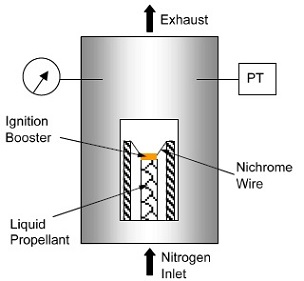
\includegraphics[width=0.75\linewidth]{Figure_1.jpg}
\caption{Schematic-Diagram of High-Pressure Optical Strand Burner. Propellant stand inserted from bottom}
\label{fig1}
\end{minipage}
\begin{minipage}{0.5\textwidth}
\centering
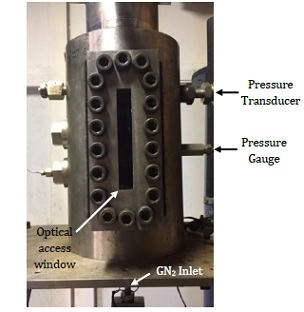
\includegraphics[width=0.75\linewidth]{Figure_2.jpg}
\caption{Photograph of High-Pressure Optical Strand Burner. Orientation shows Camera View of Optical Access Window}
\label{fig2}
\end{minipage}
\end{figure}

The maximum working pressure of the optical strand burner was 68.9 MPa (10 ksi). A constant flow of GN$_2$ was
supplied to the optical strand burner during the test to create an inert pressure environment for the propellant.
The base plate supporting the propellant had multiple feedthrough ports to provide pathways into the chamber for
electrical signal and gas lines. The viewing port of the diffuser was used for real-time recording of the burning
process by a digital video camera.

During the experiment, a small amount of AF-M315E was loaded in a borosilicate tube with 10-mm x 75-mm dimenstions
(wall thickness of $\sim$0.70-mm). The propellant level in the tube was approximately 3.175-mm below the open end.
A small sample of double-base propellant used for propellant ignition via resistively heating of a nichrome wire
was installed at the top of the propellant strand such that the double-base propellant was in physical contact with
the liquid propellant. Whether the double-base propellant was in contact, partially submerged, or fully submerged,
once the liquid propellant was ignited, burn distance data was measured after the double-base propellant was fully
consumed. To initate the double-base propellant, each end of the nichrome wire was attached to an alligator clip, 
which was routed through high-pressure feed through fittings at the bottom of the propellant strand holder. A
close-up view of an installed propellant sample is shown in Figure \ref{fig3}. In addition, AF-M315E installed in
the liquid strand burner (seen through the optical port) is shown in Figure \ref{fig4}.

\begin{figure}[htb!]
\centering
\begin{minipage}{0.5\textwidth}
\centering
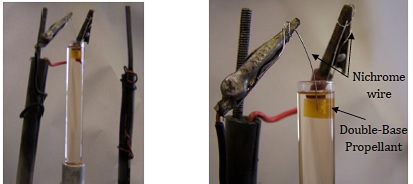
\includegraphics[width=0.75\linewidth]{Figure_3.jpg}
\caption{AF-M315E with Igniter in the Test Cylinder installed on Strand Burner Base Plate. Nichrome Wire placed through Center of Double-Base Propellant.}
\label{fig3}
\end{minipage}
\begin{minipage}{0.5\textwidth}
\centering
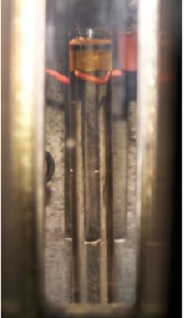
\includegraphics[width=0.75\linewidth]{Figure_4.jpg}
\caption{AF-M315E Sample seen through Front Optical Port in Liquid Strand Burner. Linear Regression of Propellant Recorded through this Optical Access Window.}
\label{fig4}
\end{minipage}
\end{figure}

For each test, video data of the combustion event was recorded with a high-speed digital camera at a framing rate
of 120 fps, capturing the propagation of the flame front as it consumes the propellant and linear regression of the
burning surface. Instrunet and LabVIEW software were used to monitor the pressure inside the strand burner chamber
as well as record instantaneous pressure and ignition data. ImageJ video software and a MATLAB data reduction code
were used to analyze the video images and calculate the linear regression burning rates with average pressure over
a selected burn time. A typical series of captured images during a combustion event is shown in Figure \ref{fig5}.

\begin{figure}[htb!]
\centering
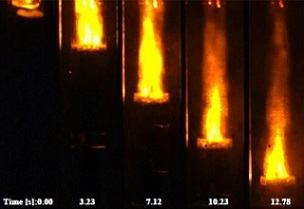
\includegraphics[width=0.25\textheight]{Figure_5.jpg}
\caption{Series of Captured Images of Linear Burning Process of AF-M315E. Demonstrates the Linear Combustion Behavior as determined form Trajectory Plots.}
\label{fig5}
\end{figure}


\section{Bayesian Inversion Analysis} \label{Bayesian_Inv_Analysis}

Bayesian Inversion methods were employed with the objectives of determining 1) the maximum likelihood estimation for
the pre-exponential coefficient $A$ and exponential $n$ of Saint-Robert's burn rate law and 2) the 95\% confidence interval 
of the model for the pressure range of interest given the data. The following sections detail the theoretical 
underpinnings utilized for the analysis of the data presented in Section \ref{Apparatus_Test} as well as the setup of QUESO.

\subsection{Theoretical Development} \label{Theory_Dev}

Theoretical development of the model was accomplished by assuming that the burn rate data is independent and 
identically distributed, the likelihood probability density function of the burn rate is Gaussian, the prior 
is uniform and the error is additive. These assumption led to Equation \ref{add_err}. 

\begin{equation} \label{add_err}
R_b (P)=R_b (P)_{mle} + \varepsilon (P)
\end{equation}

Saint-Robert's burning law ($R_b=A \cdot P^n$) was linearized by taking the natural log of both sides of Eq. \ref{add_err}.

\begin{equation} \label{ln_st_rob}
L(P) = \ln [R_b(P)] = \ln (A) + n \cdot \ln (P)
\end{equation}

Applying the assumptions simplified the posterior probability density function to the following equation:

\begin{equation} \label{prob}
prob( \vect{X} |D, I) \propto \frac{1}{\sigma_k \sqrt{2 \pi} } \cdot \exp{\bigg( \frac{-[L(P)-\ln(D_k)]^2}{2\sigma_k^2} \bigg)}
\end{equation}

In Eq. \ref{prob}, $\vect{X}$ denotes the vector of parameters $\ln(A)$ and $n$ (i.e. $\vect{X}=[\ln(A) \quad n]^T$). 
The analysis also assumed that $\sigma_k$ was constant and determined from the covariance ($\sigma^2$) during the MCMC 
Metropolis-Hastings investigation of the resulting probability density function.

The 95\% confidence interval ($2\sigma$) was evaluated by applying the definition for a Gaussian probability density distribution 
to the linearized model for burn rate as shown in Eq. \ref{kpequ}

\begin{equation} \label{kpequ}
K(P)=N(\vect{X}_{mle},\sigma_k^2) \sim N(\vect{X}_{mle}, \vect{F}^T V \vect{F})
\end{equation}

In Eq. \ref{kpequ}, V is the resultant covariance matrix of the MCMC Metropolis-Hastings analysis and $\vect{F}$, a function of
pressure P, is a vector of the coefficients for the parameters of the linearized Saint-Robert's burning law and is given by
Eq. \ref{FP_equ}.

\begin{equation} \label{FP_equ}
\vect{F}(P)= 
\begin{bmatrix}
1 \\ 
\ln(P)
\end{bmatrix}
\end{equation}

It can be seen by inspection that $K(P) = \ln[R_b(P)]$ can be recovered using Eq. \ref{KP_equ2}.

\begin{equation} \label{KP_equ2}
K(P) = \ln[R_b(P)] = \vect{F}(P) \cdot \vect{X} = [1 \quad \ln(P)] \cdot 
\begin{bmatrix}
\ln(A) \\ 
n
\end{bmatrix}
\end{equation}

The variance from Eq. \ref{kpequ} can be calculated in Eq. \ref{var} since the model is linear.

\begin{equation} \label{var}
\sigma^2 = \vect{F}(P)^T \cdot V \cdot \vect{F}(P)
\end{equation}

Therefore, the 95\% confidence interval for the burn rate of the candidate ionic liquid propellant can now be determined
using Eqs. \ref{ln_st_rob} and \ref{var} where $\varepsilon = \sqrt{\sigma^2}$ and the 95\% confidence interval is 
defined as $2\sigma$.

\begin{equation} \label{Rb95}
R_b(P)_{95\% Confidence} = \exp{(L(P)_{mle} \pm 2 \sqrt{\sigma^2})}
\end{equation}

\subsection{QUESO Setup} \label{QUESO_setup}

QUESO was set up to determine the values of the parameters of Saint-Robert's burning law and their uncertainty.
This was accomplished by first utilizing GNU's Scientific Library (GSL) Nelder-Mead2 optimization algorithm to 
calculate the maximum likelihood estimates (mle) of the parameters $\ln(A)$ and $n$ assuming a Gaussian likelihood. 
A maximum of 1000 iterations were allowed in determining the optimized values of $\ln(A)$ and $n$ with a maximum 
tolerance of $10^{-10}$. 

The uncertainty in the parameters was determined by utilizing QUESO's Bayesian Inverse Problem Metropolis-Hasting 
DRAM algorithm. A raw chain size of $10^7$ was requested as well as a filtered chain with a lag of 250. The initial 
proposal covariance matrix was set to $diag[10 \quad 10]$. All QUESO analysis runs utilized the same QUESO input 
options with the exception of a directive to where the results of each analysis were stored.

\section{Results \& Discussion} \label{results}

\subsection{Experimental Strand Burner Data} \label{resultsExpr}

A series of strand burner experiments over an average chamber pressure range of 0 - 1000 psig was conducted for 
AF-M315E to determine the burning rate as a function of pressure. Based upon the results, AF-M315E demonstrated
self-sustained burning behavior over an average chamber pressure range of 300 - 1000 psia. Below an average 
chamber pressure of 470 psia, AF-M315E did not sustain continuouse, self-deflagration behavior. During tests
conducted at average pressures of 315, 437 and 465 psia, AF-M315E burned for a small portion of time and then
self-quenched (i.e. stopped burning); however, at an average pressure of 469 psia, continuous self-sustained
burning occured. Therefore, it is believed that an average chamber pressure around 470 psia was the pressure
deflagration limit (PDL) for AF-M315E. However, in order to fully identify the PDL, a series of experiments 
should be conducted in the future at discrete, incremental pressure levels between 450 and 470 psia.

Examples of trajectory plots, that is, the burning surface position as a function of time, is given in Figure
\ref{fig6}. Figure \ref{fig6} exhibits the trajectory plot comparing the effect of pressure on the burning rate
for AF-M315E. The data for three average chamber pressures 556, 782 and 1008 psia are shown. High-quality linear
fits were applied to the data to attain yielding burning rates of 1.42, 2.39 and 4.00 mm/s, respectively, for
the three average chamber pressures.

\begin{figure}[htb!]
\centering
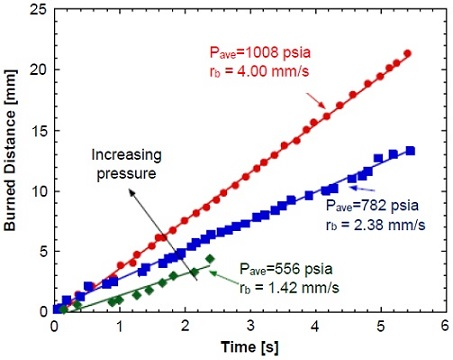
\includegraphics[width=0.25\textheight]{Figure_6.jpg}
\caption{Burned Distance of AF-M315E as a function of time at Mulitple Pressures. Higher Pressures led to Increased Burned Distance.}
\label{fig6}
\end{figure}

The complete burns of AF-M315E are shown in Figure \ref{fig7}. A number of experiments were conducted around 700
psia and no deflaration was observed. The reason for this phenomenon is not fully clear, but may be attributed to
aging of the propellant. From approximately 470 to 650 psia, a plateau region of complete burning was observed. As
can be seen from Figure \ref{fig7}, each region resulted in a burn rate power fit for AF-M315E as a function of 
average chamber pressure (i.e. Saint-Robert's burning law). Additional tests above 1000 psia were conducted to
determine if there was any slope break in burn rate at higher pressures. There was not. The resulting burn rates 
for AF-M315E can be seen in Eqs. \ref{hp_Rb_exp} \& \ref{lp_Rb_exp}. 

\begin{equation} \label{hp_Rb_exp}
For 780 - 1600 psia:	R_b=5.01x10^{-6} \cdot P^{1.96}
\end{equation}

\begin{equation} \label{lp_Rb_exp}
For 470 - 650 psia:	R_b=1.78 \cdot P^{-0.0386}
\end{equation}


\subsection{Bayesian Inversion Analysis} \label{resultsBayes}

The experimental burn rate data was analyzed applying two assumptions. The first assumed
that all the data could be accurately model using a single Saint-Robert's burning law. The second 
assumes that two Saint-Robert's burning laws accurately modeled the data; one for the low pressure 
regime (300 psi to 650 psi) and a second for higher pressure (780 psi to 2000 psi). This 
second assumption is identical to the linear regression fit performed by the experimenters. The assumption
seemed reasonable due to the fact that an intermediate 
pressure regime (650 psi to 780 psi) where the propellant self-extinguished. This behavior 
could indicate that the relative rates between intermediate reactions is changing in each 
pressure regime and may not be well characterized by a single Saint-Robert's burning law. 
The results based on these assumptions are discussed in of the following sections.

\subsection{Single Burn Rate Law Model} \label{singleRate}

Assuming a single burn rate law could model the observed data resulted in $A$ and $n$ equal 
to 0.9674 and 1.9046, respectively. As can be seen in Figure \ref{SingleBRfig}, this 
results in a burn rate model that fits well with burn rates recorded at pressures $\geq$780 psi.
It does not appear to model the burn rates recorded at pressures $<$780 psi. 
Based on this result, it was conclude that two burn rate laws would model the data better. 
As such, further analysis on this model was not pursued.

\begin{figure}[htb!]
\centering
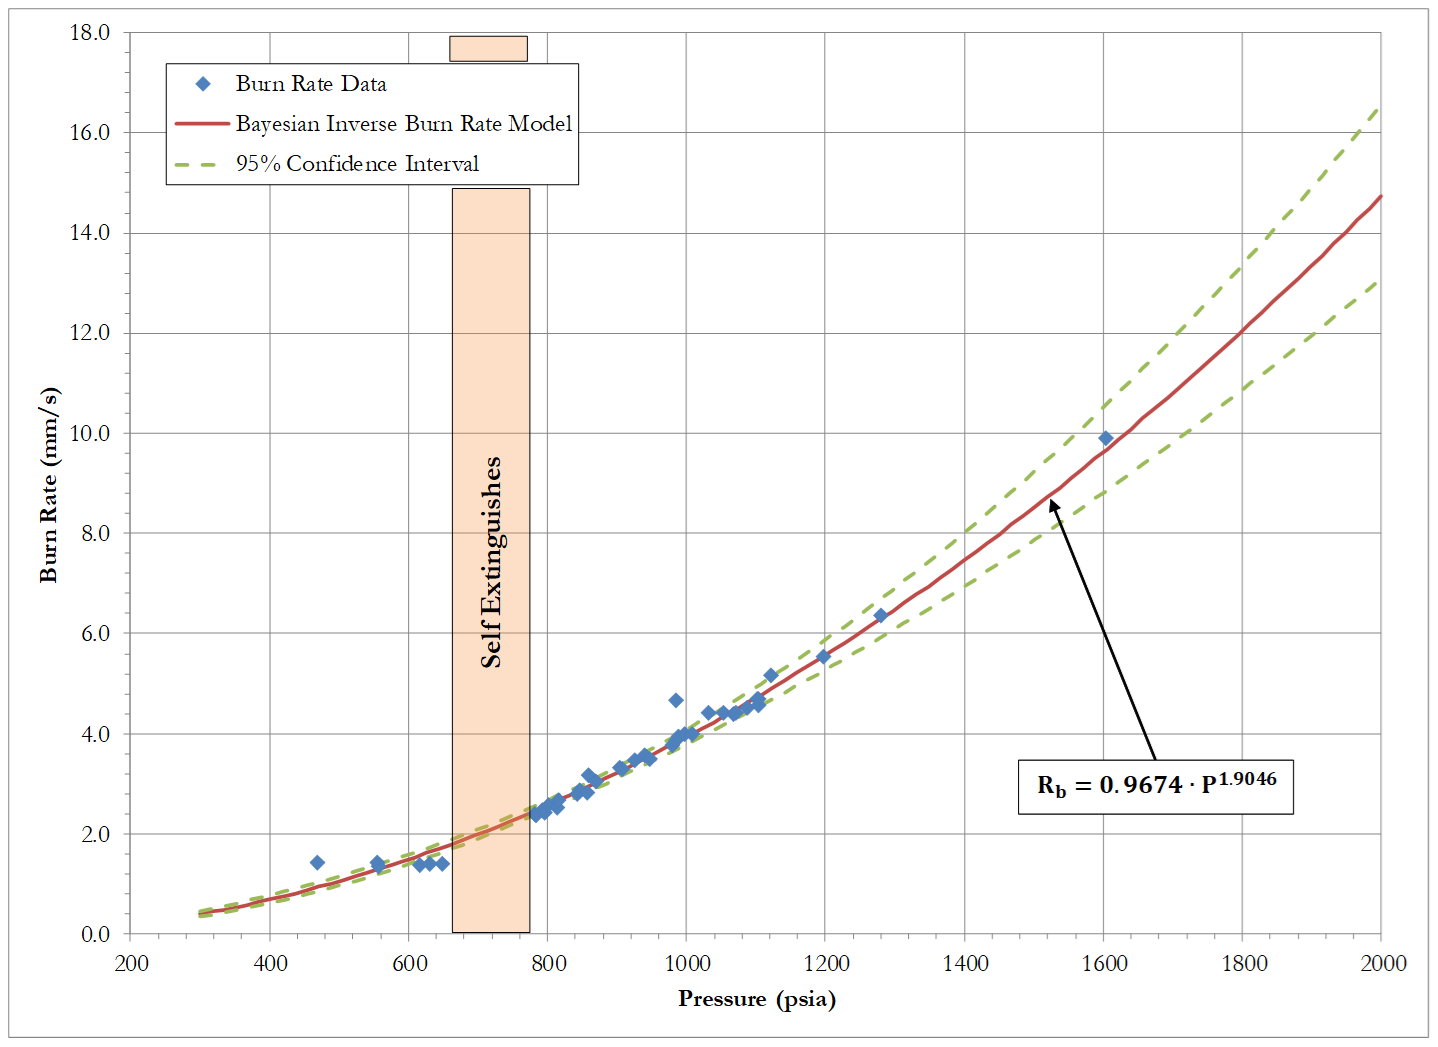
\includegraphics[width=0.25\textheight]{Single_Burn_Rate_Results.png}
\caption{Single Burn Rate Law Model \& Data Comparison. Model Accurate at Pressures above Self-Extinguished Zone.}
\label{SingleBRfig}
\end{figure}

\subsection{Dual Burn Rate Law Model} \label{twoBurnRateResults}

Based upon the inaccuracy in the single model assumption, the experimental burn rate data was modeled
as a dual burn rate law. The resulting burn rate constants $A$ and $n$ can be seen in Table
\ref{Table:brlpresults} for both pressure regimes. 

\begin{table}
\centering
\caption{Burn Rate Law Parameter Results}
\label{Table:brlpresults}
\begin{tabular}{|c|c|c|c|c|}
\hline
Parameter & \multicolumn{2}{|c|}{Bayesian Analysis} & \multicolumn{2}{|c|}{Experimenter's Regression} \\ \cline{2-5}
 & Low Pressure & High Pressure & Low Pressure & High Pressure \\ \hline
$A$ & 1.1880 & $5.1131 \cdot 10^{-6}$ & 1.78 & $5.01 \cdot 10^{-6}$ \\ \hline
$n$ & 0.0215 & 1.9631 & -0.0386 & 1.96 \\
\hline
\end{tabular}
\end{table}

This current analysis using Bayesian Inversion methods agreed well in the high pressure regime. However, the
results shows that the current analysis varies appreciably from the experimental linear regression in the low
pressure regime. The resulting Bayesian Inversion Method models have tight 95\% confidence intervals in 
areas where the data is more concentrated. Figure \ref{DualBRfig} shows the resulting models and 95\% confidence 
intervals compared to the recorded data.

\begin{figure}[htb!]
\centering
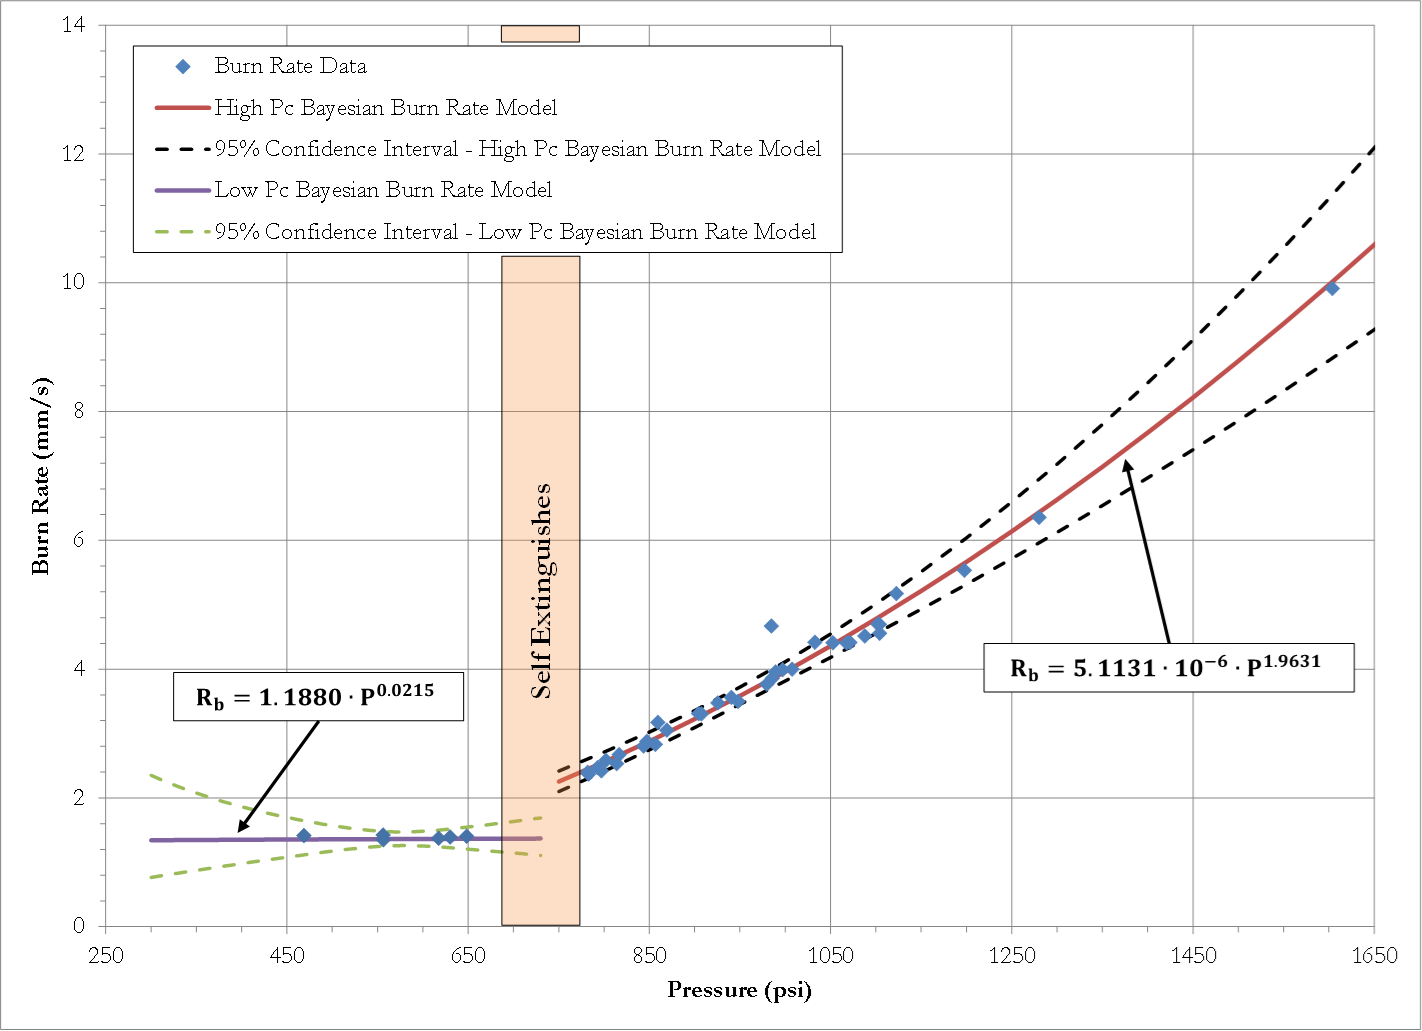
\includegraphics[width=0.25\textheight]{Dual_Burn_Rate_Results.png}
\caption{Dual Burn Rate Law Model \& Data Comparison. Model Accurately Predicts Burn Rate for AF-M315E.}
\label{DualBRfig}
\end{figure}

Uncertainty quantification of the burn rate model parameters were investigated using QUESO's Metropolis-Hastings
algorithm. Before providing the resulting Parameter Density Functions (pdf) for each of the parameters in each of 
the models, a plot of the filtered chain is provided in Figures \ref{LPChain} \& \ref{HPChain}. As expected, 
plots which resemble white noise were generated. Additionally, the filtered sampling chains were analyzed for
autocorrelation using MATLAB's autocorr function. Again, as expected, the Autocorrelation Functions (ACF) shown in
Figures \ref{autoHP} \& \ref{autoLP} decrease and tend to zero as lag increases. Together these results indicate
random samplings of the pdf for each of the parameters.

\begin{figure}[htb!]
\centering
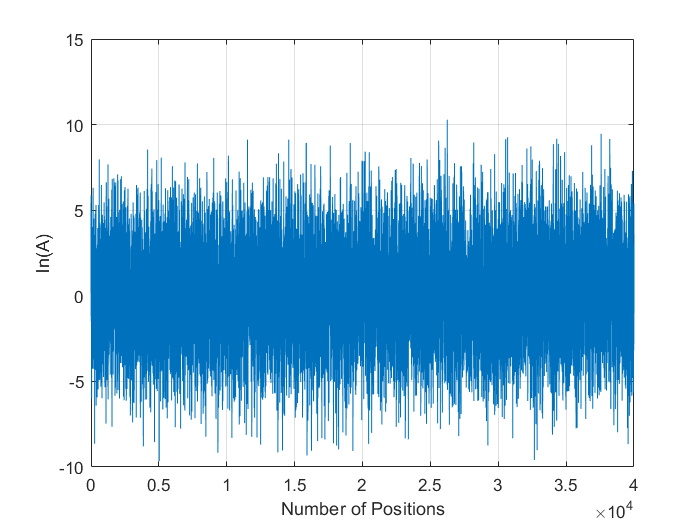
\includegraphics[width=0.48\textwidth]{FilteredChain_lnA_LP.png}
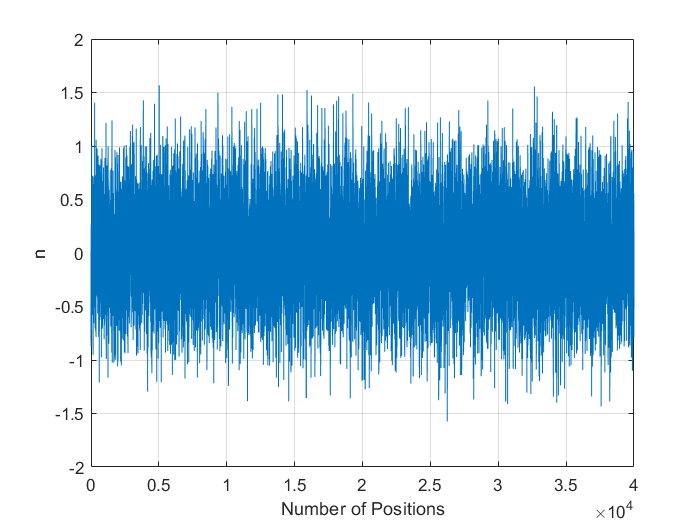
\includegraphics[width=0.48\textwidth]{FilteredChain_n_LP.png}
\caption{Filtered Chain Plot - Low Pressure Model Parameters}
\label{LPChain}
\end{figure}

\begin{figure}[htb!]
\centering
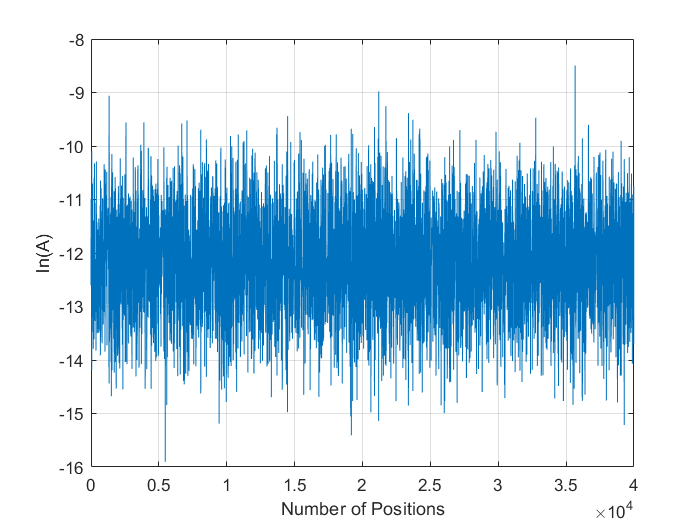
\includegraphics[width=0.48\textwidth]{FilteredChain_lnA_HP.png}
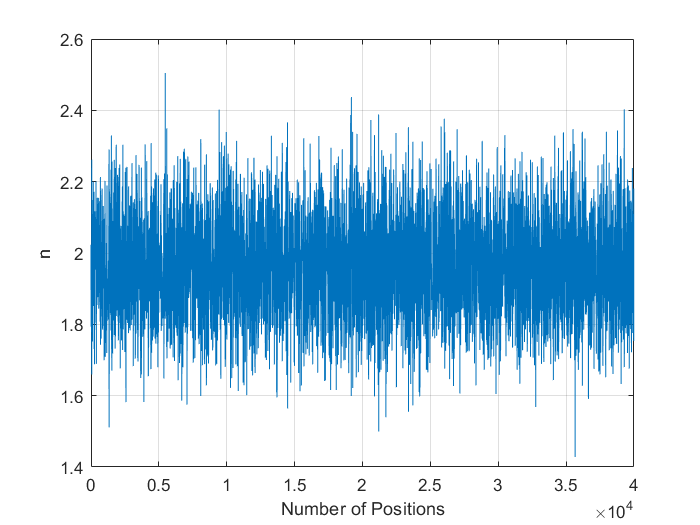
\includegraphics[width=0.48\textwidth]{FilteredChain_n_HP.png}
\caption{Filtered Chain Plot - High Pressure Model Parameters}
\label{HPChain}
\end{figure}

\begin{figure}[htb!]
\centering
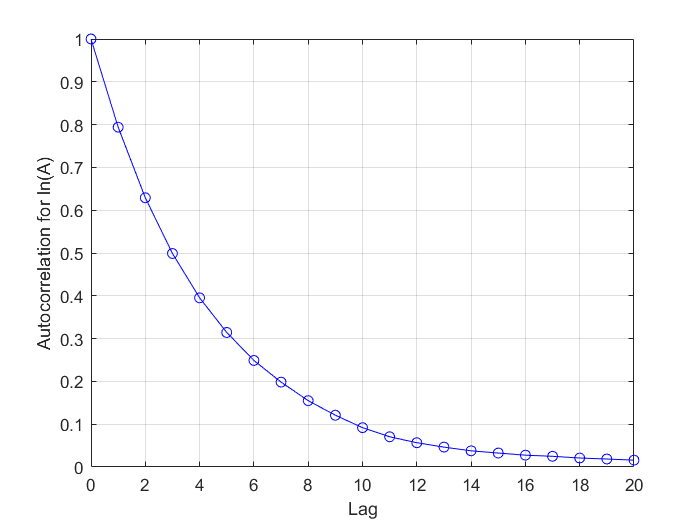
\includegraphics[width=0.48\textwidth]{ACF_lnA_filt_HP.png}
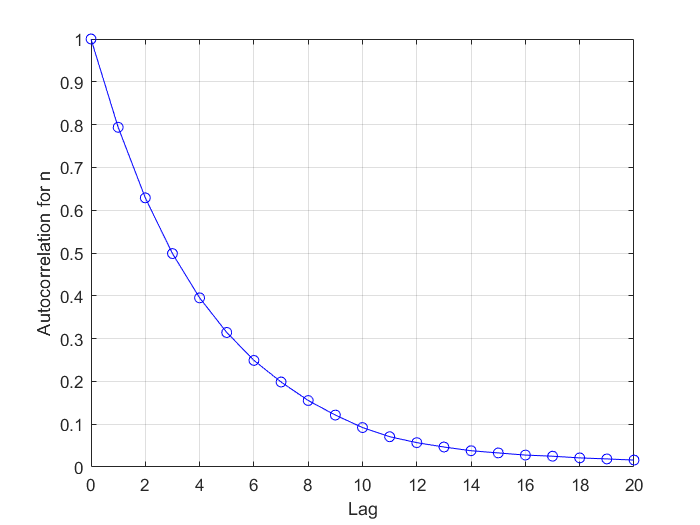
\includegraphics[width=0.48\textwidth]{ACF_n_filt_HP.png}
\caption{Filtered Chain High Pressure ACF v Lag}
\label{autoHP}
\end{figure}

\begin{figure}[htb!]
\centering
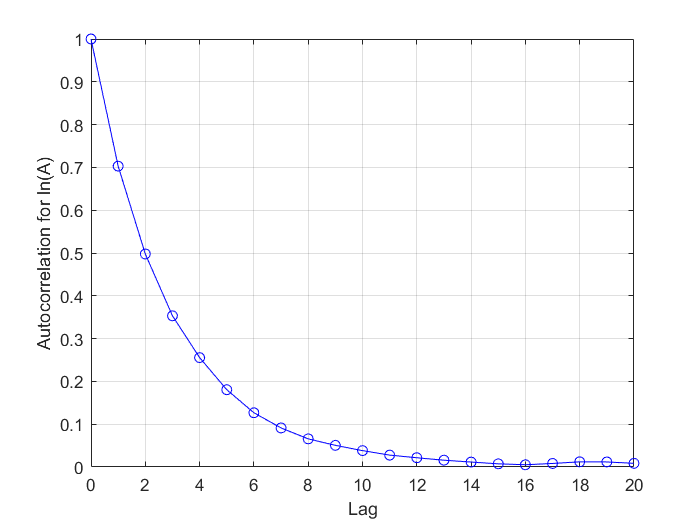
\includegraphics[width=0.48\textwidth]{ACF_lnA_filt_LP.png}
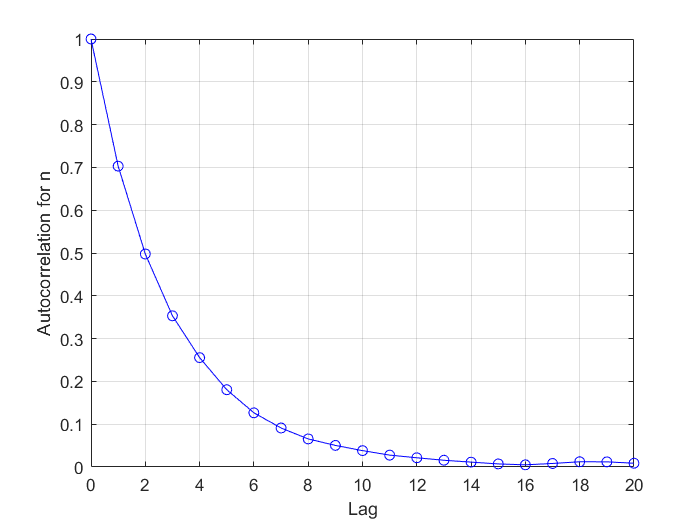
\includegraphics[width=0.48\textwidth]{ACF_n_filt_LP.png}
\caption{Filtered Chain Low Pressure ACF v Lag}
\label{autoLP}
\end{figure}

The pdf's for each of the model parameters are provided in Figures \ref{LPpdf} \& \ref{HPpdf}. These figures show that each of 
the parameters' uncertainties have been captured within the -100 to 100 range of the parameter space and show 
a traditional Gaussian profile. The singular peak is reasonably concentrated for each pressure regime model's 
parameter considering the limited number of data points available (9 data points in the low pressure regime, 
35 data points in the high pressure regime). Including additional data in each of the pressure regimes
is expected to result in smaller variance which would manifest itself as a narrower Guassian pdf profile with an even
more concentrated, well-defined peak.

\begin{figure}[htb!]
\centering
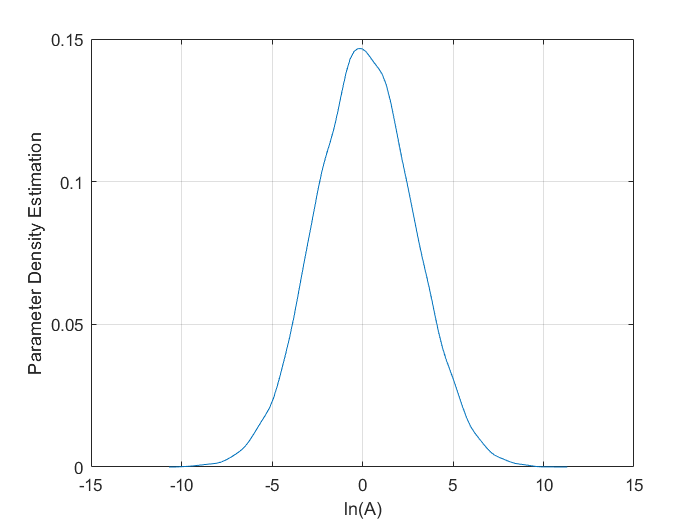
\includegraphics[width=0.48\textwidth]{PDF_lnA_LP.png}
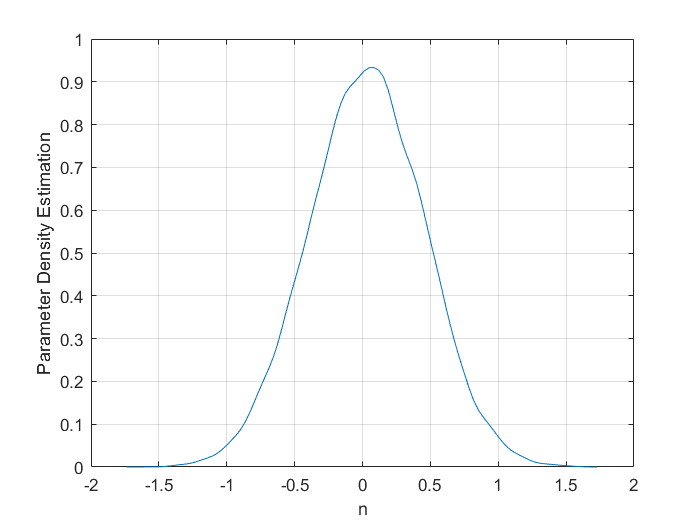
\includegraphics[width=0.48\textwidth]{PDF_n_LP.png}
\caption{Resulting Parameter Density Function - Low Pressure Model Parameters}
\label{LPpdf}
\end{figure}

\begin{figure}[htb!]
\centering
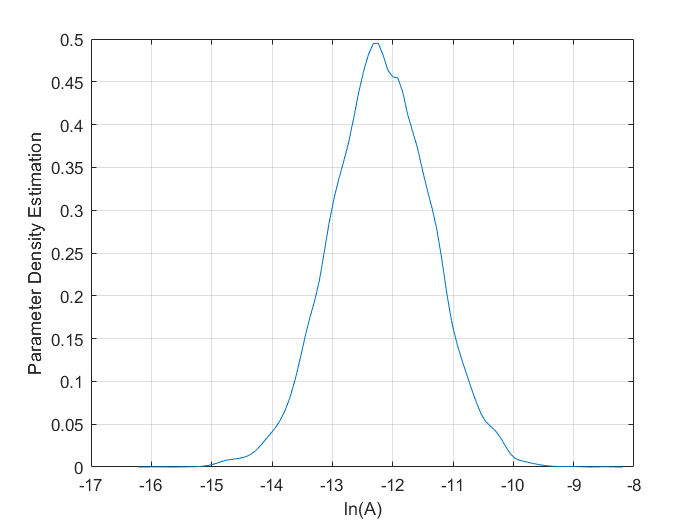
\includegraphics[width=0.48\textwidth]{PDF_lnA_HP.png}
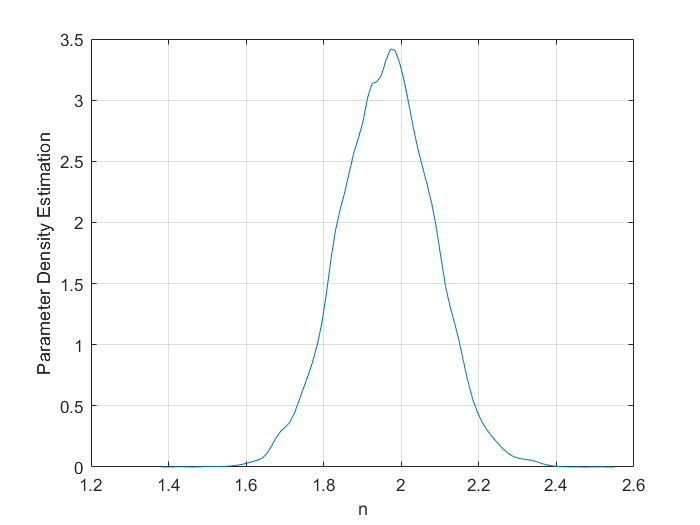
\includegraphics[width=0.48\textwidth]{PDF_n_HP.png}
\caption{Resulting Parameter Density Function - High Pressure Model Parameters}
\label{HPpdf}
\end{figure}

Overall, the results show that the Bayesian Inversion methods employed for this analysis provided additional information
about the burn rate of AF-M315E which was not provided and/or determined by experimental data. The "for-free" ability to
determine the 95% confidence interval from the convariance allows one to a) determine what pressure regimes to collect
additonal data to improve the models and b) if those experiments were executed, the range over which one would most likely
expect the burn rate to be. This knowledge would allow experimenters in the future to determine if the result was expected
and may indicate that there was something erroneous with the measurement or if the propellant was entering a new burn rate
regime from simple inspection of the figures. Both pieces of information would allow for better decisions to be made in
both determining what to test and assessing the observation in-situ.

\section{Conclusion} \label{conclusion}

A comparison between the experimental burn rate model and the resulting Bayesian Inversion model for ionic liquid
AF-M315E was conducted. Analysis showed that applying two Saint-Robert's burning law models, one for low pressure
(300 - 650 psi) and one for high pressure (780 - 2000 psi), to predict the burn rate of AF-M315E was more accurate
and represented the data better than a single Saint-Robert's burning law. This was consistent with the experimental
linear regression model of the data. The models agreed well for the high pressure regime, but differed at the low
pressure regime. They particularly diverge in their slope at the low pressure regime, with the experimental burn
rate model having a negative slope and the burn rate model inferred useing Bayesian Invserion methods having a positive
slope. The expectation is for the burn rate to increase as the pressure increases (i.e. as molecular collision frequencies
increase, the burn rate of the propellant increases). The Bayesian Inversion burn rate model supported this hypothesis.
On the other hand, there is a marked pressure regime (650 psi $\leq P \leq$ 780 psi) where the propellant self-extinguishes.
The negative slope put forth by the experimental data may be an indicator of this behavior. It is possible that the
experimental data model and Bayesian Inversion model presented may converge with the availability of additional data
in the low pressure regime (i.e. only 9 data points were observed).

\nocite{*}
\bibliography{burnRateBib}
\bibliographystyle{plain}

\end{document}

